\subsection{CLion konfigurieren}
Wenn CLion als IDE verwendet wird, so müssen die folgenden Schritte durchgeführt werden.
In einem ersten Schritt wird CLion geöffnet und über 'File - New Project' ein neues Projekt ersetllt.
Nun muss das höchste CMakeLists.txt file des Repositorys 'learn\textunderscore with\textunderscore tello' ausgewählt werden.
Danach kann die Build-Umgebung eingerichtet werden.

\begin{itemize}
    \item Öffne 'File - Settings'
    \item Navigiere zu 'Build, Execution, Deployment'
    \item Wähle 'Toolchains' aus
    \item Prüfe, ob eine Toolchain namens 'Visual Studio' verfügbar ist.
    Wenn ja, erübrigen sich die weiteren Schritte.
    \item Drücke den 'Add'-Button in der oberen linken Ecke
    \item Nun muss die Umgebung ausgewählt werden. Beachte das nachfolgende Bild.
    Es muss mindestens eine CMake-Version 3.18.2 verfügbar sein.\par
    \begin{minipage}{\linewidth}
        \centering
        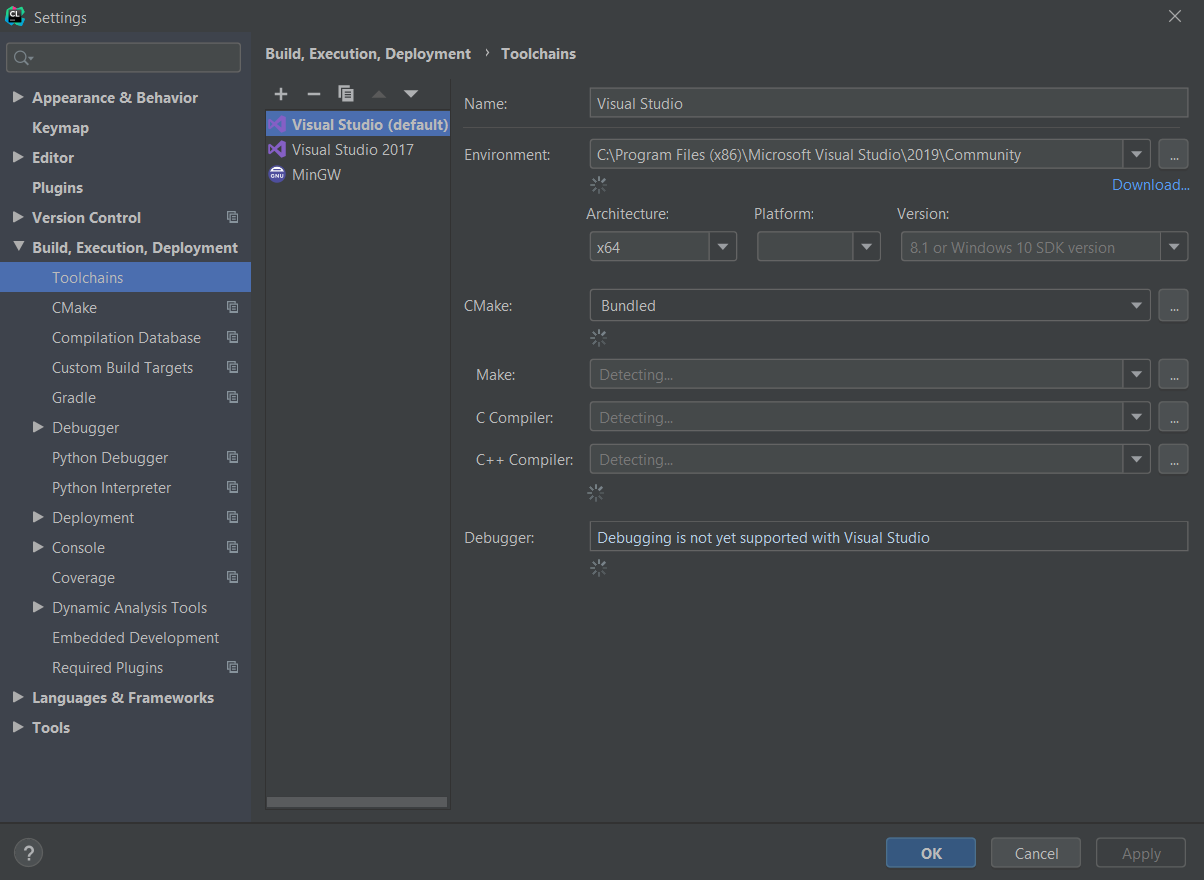
\includegraphics[width=0.6\textwidth]{../common/chapter_01/resources/01_clion_configure_toolchain.png}
        \captionof{figure}{CLion toolchain Konfiguration}
    \end{minipage}
\end{itemize}
Nun bist du in der Lage, das Projekt im 'Debug'-Modus zu erstellen. Damit ist gemeint, dass zu jeder Library oder jeder
ausführbaren-Datei (executable) zusätzlicher Code der Applikation hinzugefügt wird. Dadurch wird das Binary ungefähr zehn mal langsamer.
Wenn du die Applikation im Release-Modus erstellen willst, dann musst du die folgenden Schritte durchführen.
Im Release-Modus kann eine Applikation nicht mehr schrittweise durchlaufen werden, dafür ist sie viel performanter.
Dieser Modus wird verwendet, wenn eine Applikation fertig ist und sich nicht mehr in der Entwicklungsphase befindet.
\begin{itemize}
    \item Öffne 'File - Settings'
    \item Navigiere nach 'Build, Execution, Deployment'
    \item Wähle 'CMake' aus
    \item Prüfe, ob ein Profil namens 'Release' verfügbar ist. Wenn ja, dann ist bereits alles eingerichtet.
    \item Drücke den 'Add'-Button in der oberen linken Ecke.
    \item Ein neuer Eintrag wird erstellt. Benenne ihn 'Release', wenn dies nicht schon der Fall ist.
\end{itemize}
Nun werden die CMake-Konfigurationen neu erstellt. Nach diesem Vorgang, kannst du einen Blick in die obere rechte Ecke
von CLion werfen. Dort siehst du ein grünes Hammersymbol. Daneben befindet sich ein Dropdown, wo die verschiedenen
'targets' (Ziele) ausgewählt werden können. Die Konfiguration wird dahinter ausgegeben. Dies ist entweder 'Debug' oder
'Release'. Wenn du das Dropdown ausklappst, kannst du sehen, dass du zwischen diesen Konfigurationen 'Debug' und 'Release'
sowie allen 'targets' wechseln kannst. Ein 'target' wird in diesem Kontext als library oder executable-file verstanden.
Es kann aber auch etwas spezielleres sein wie zum Beispiel ein Vorgang, um Dateien von einem Verzeichnis in ein anderes
zu kopieren.\\
Die folgenden 'targets' sollten vorhanden sein (Es werden nicht alle aufgeführt):
\begin{description}
    \item[00\textunderscore base\textunderscore module] Beinhaltet Basiseinstellungen für die Drohne(n)
    \item[01\textunderscore keyboard\textunderscore module] Die ersten paar Übungen.
    \item[01\textunderscore keyboard\textunderscore module\textunderscore solution] Die Lösungen zu den Übungen.
    \item[99\textunderscore template] Dies ist eine Vorlage für neue Module, das kann ignoriert werden.
    \item[app\textunderscore basic] Die Hauptapplikation (Um diese zu starten, drücke den grünen Play-Button hinter dem Dropdown mit den 'targets')
    \item[app\textunderscore common] Eine Bibliothek mit Code, den alle Module verwenden.
    \item[app\textunderscore common\textunderscore video] Eine Bibliothek mit Code, den Module verwenden können.
\end{description}
Um ein 'target' zu kompilieren, muss dieses im Dropdown ausgewählt werden. Danach wird der grüne Hammer daneben
geklickt. Für den Anfang reicht es, wenn die folgenden 'targets' erstellt werden:
\begin{itemize}
    \item app\textunderscore basic
    \item 00\textunderscore base\textunderscore module
    \item 01\textunderscore keyboard\textunderscore module
\end{itemize}
Wenn die Builds allesamt ohne Fehler durchlaufen, dann kannst du deine Tello-EDU-Drohne starten.
Du solltest sie zuerst mit der offiziellen App kalibrieren.
Stelle sie danach auf den Boden, wo genug Platz drumherum und nach oben ist. Die Drohne sollte gelb blinken, das heisst,
sie wartet auf eine Verbindung. Wähle in den WLAN-Einstellungen das Tello-EDU WLAN aus.\\
Wähle nun das 'target' 'app\textunderscore basic' aus und drücke den Play-Button. Um deine Umgebung zu testen, drücke
den Button 'Take off' in der Applikation. Wenn die Drohne fliegt und du ein Bild siehst, hast du alles richtig gemacht
und kannst nun mit den Übungen starten. Drücke den Knopf nochmals, um die Drohne zu landen und schliesse die Applikation.